\chapter{Evaluation}
\label{chp:chapter_4}

This chapter describes the process of evaluating the optimizations and the results of said evaluations.

\section{Setup}
\label{sec:evaluation_setup}

Blah blah blah evaluation setup

\section{Results}
\label{sec:evaluation_results}


% Number of Packets Plot
\pgfplotsset{
    compat=1.9,
    compat/bar nodes=1.8,
}
\pgfplotstableread{
    Label Discovery Configuration Link-layer emptypdu Application
    0     58        8             9          6        2
    1     58        8             9          7        2
    2     6         8             9          10       5
    3     0         0             9          3        5
    4     0         0             1          0        0
}\connsetupdata
\begin{figure}
    \begin{center}
    \begin{tikzpicture}
        \begin{axis}[
            ybar stacked,
            ymin=0,
            ymax=100,
            xtick=data,
            legend style={
                cells={anchor=west},
                legend pos=north east,
            },
            reverse legend=true,
            xticklabels from table={\connsetupdata}{Label},
            xticklabel style={text width=2cm,align=center},
        ]
            \addplot [fill=green!80]
                table [y=Discovery, meta=Label, x expr=\coordindex]
                    {\connsetupdata};
                        \addlegendentry{Discovery}
            \addplot [fill=blue!60]
                table [y=Configuration, meta=Label, x expr=\coordindex]
                    {\connsetupdata};
                        \addlegendentry{Configuration}
            \addplot [fill=red!60]
                table [y=Link-layer, meta=Label, x expr=\coordindex]
                    {\connsetupdata};
                        \addlegendentry{Link Layer}
            \addplot [fill=gray!60]
                table [y=emptypdu, meta=Label, x expr=\coordindex]
                    {\connsetupdata};
                        \addlegendentry{Empty PDU}
            \addplot [fill=purple!60,nodes near coords,point meta=y]
                table [y=Application, meta=Label, x expr=\coordindex]
                    {\connsetupdata};
                        \addlegendentry{Application}
        \end{axis}
    \end{tikzpicture}
\end{center}
\caption{Division of Packets for Levels of Optimization}
\label{fig:division_packets}
\end{figure}


% Setup Time Plot
\pgfplotsset{
    compat=1.9,
    compat/bar nodes=1.8,
}
\pgfplotstableread{
    Label SetupTime 
    0     1.862        
    1     134.762     
    2     37.591   
    3     15.997    
    4     0.001    
}\setuptimedata
\begin{figure}
    \begin{center}
\begin{tikzpicture}
    \begin{axis}[
        ybar,
        ymin=0,
        ymax=150,
        xtick=data,
        xticklabels from table={\setuptimedata}{Label},
        xticklabel style={text width=2cm,align=center},
    ]
        \addplot [fill=green!60,nodes near coords,point meta=y]
            table [y=SetupTime, meta=Label, x expr=\coordindex]
                {\setuptimedata};
    \end{axis}
\end{tikzpicture}
\end{center}
\caption{Connection Setup Time}
\end{figure}

% Time To Useful Packet Plot
\pgfplotsset{
    compat=1.9,
    compat/bar nodes=1.8,
}
\pgfplotstableread{
    Label Time 
    0     5.021
    1     136.762  
    2     25.994
    3     4.800
    4     6.445
}\timetousefuldata
\begin{figure}
    \begin{center}
        \begin{tikzpicture}
            \begin{axis}[
                ybar,
                ymin=0,
                ymax=150,
                xtick=data,
                xticklabels from table={\timetousefuldata}{Label},
                xticklabel style={text width=2cm,align=center},
            ]
                \addplot [fill=blue!60,nodes near coords,point meta=y]
                    table [y=Time, meta=Label, x expr=\coordindex]
                        {\timetousefuldata};
            \end{axis}
        \end{tikzpicture}
    \end{center}
    \caption{Time Until Useful Packet}
\end{figure}


% Connection Adaption Time vs. current CI
\begin{figure}
    \begin{center}
    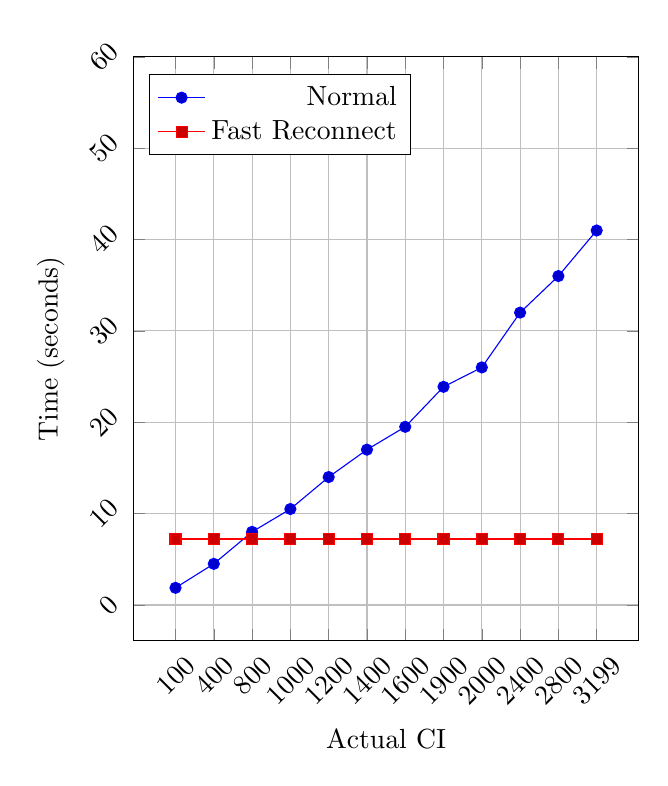
\begin{tikzpicture}
    \begin{axis}[
    ymax = 60,
    symbolic x coords={100, 400, 800, 1000, 1200, 1400, 1600, 1900, 2000, 2400, 2800, 3199},
    xtick=data,
    height=9cm,
    width=8cm,
    grid=major,
    xlabel={Actual CI},
    ylabel={Time (seconds)},
    legend style={
    cells={anchor=east},
    legend pos=north west,
    tick label style={rotate=45} % <-- this is added
    }
    ]
    
    \addplot coordinates {
        (100,1.875)
        (400,4.5)
        (800,8)
        (1000,10.5)
        (1200,14)
        (1400,17)
        (1600,19.5)
        (1900,23.876)
        (2000,26)
        (2400,32)
        (2800,36)
        (3199,40.989)
    };
    \addplot coordinates {
        (100,7.22)
        (400,7.22)
        (800,7.22)
        (1000,7.22)
        (1200,7.22)
        (1400,7.22)
        (1600,7.22)
        (1900,7.22)
        (2000,7.22)
        (2400,7.22)
        (2800,7.22)
        (3199,7.22)
    };
    
    
    \legend{Normal, Fast Reconnect}
\end{axis}
\end{tikzpicture}
\end{center}
        \caption{Connection Adaption Time}
\end{figure}